\documentclass[aspectratio=169]{beamer}
\usetheme{Madrid}

% Theme
% \definecolor{TAMMaroon}{RGB}{80,0,0}
% \usecolortheme[named=TAMMaroon]{structure}

% Packages
\usepackage{graphicx}
\usepackage{listings}
\usepackage{hyperref}
\usepackage{booktabs}
\usepackage{ulem} % --> for underline
\usepackage{multicol} % --> for two-col agenda
\usepackage{subcaption}

\title{
Making Acoustic Side-Channel Attacks on Noisy Keyboards Viable with LLM-Assisted Spectrograms' ``Typo'' Correction
}
% \subtitle{}
\author{
  \underline{Seyyed Ali Ayati}\inst{1} \and 
  Jin Hyun Park\inst{1} \and 
  Yichen Cai\inst{2} \and 
  Marcus Botacin\inst{1}
}

\institute{
  \inst{1} Texas A\&M University \\
  \inst{2} University of Toronto
}

\date{
USENIX WOOT'25\\
Seattle, WA\\[0.5em]
\texttt{\href{mailto:ali.a@tamu.edu}{ali.a@tamu.edu}}
}

\titlegraphic{
  \raggedright
  
\includegraphics[height=0.8cm]{figures/CSCE_horiz.png}
}

% Footer Settings
\setbeamertemplate{footline}{
  \leavevmode%
  \hbox{%
    \begin{beamercolorbox}[wd=0.3\paperwidth,ht=2.5ex,dp=1.5ex,left, leftskip=1em]{author in head/foot}%
      \usebeamerfont{author in head/foot}Texas A\&M University
    \end{beamercolorbox}%
    \begin{beamercolorbox}[wd=0.4\paperwidth,ht=2.5ex,dp=1.5ex,center]{author in head/foot}%
      \usebeamerfont{author in head/foot}USENIX WOOT 2025
    \end{beamercolorbox}%
    \begin{beamercolorbox}[wd=0.3\paperwidth,ht=2.5ex,dp=1.5ex,right,rightskip=1em]{author in head/foot}%
      \usebeamerfont{author in head/foot}\insertframenumber{} / \inserttotalframenumber
    \end{beamercolorbox}%
  }%
}

% \setbeamertemplate{headline}{
%   \leavevmode%
%   \hbox{%
%     \begin{beamercolorbox}[wd=\paperwidth,ht=2.5ex,dp=1.5ex,leftskip=1em]{section in head/foot}
%       \usebeamerfont{section in head/foot}\insertsectionhead~\textgreater~\insertsubsectionhead
%     \end{beamercolorbox}%
%   }
% }


\setbeamertemplate{caption}[numbered]

\begin{document}
%% -------------------------------------------------------
\frame{\titlepage}
%% -------------------------------------------------------
\begin{frame}{Agenda}
  \begin{multicols}{2}
    \tableofcontents[sections={1-2}]
    \columnbreak
    \tableofcontents[sections={3-4}]
  \end{multicols}
\end{frame}
%% -------------------------------------------------------
\section{Introduction}
\subsection{Why ASCAs still matter more than ever!?}
\begin{frame}{Is This a Good Password?}
  \begin{center}
    {\Huge\ttfamily Lw7@NcQhZ\#f8GvXsT2rY}
  \end{center}
\end{frame}
%% -------------------------------------------------------
\begin{frame}{Passwords Are Gone!}
  \begin{columns}[c] % align vertically center
    \begin{column}{0.6\textwidth}
      \begin{itemize}
        \item This is a strong password.
        \item But can you remember it? Most people can’t.
        \item So we switched to something better…
      \end{itemize}
    \end{column}
    \begin{column}{0.4\textwidth}
      \begin{figure}
        \centering
        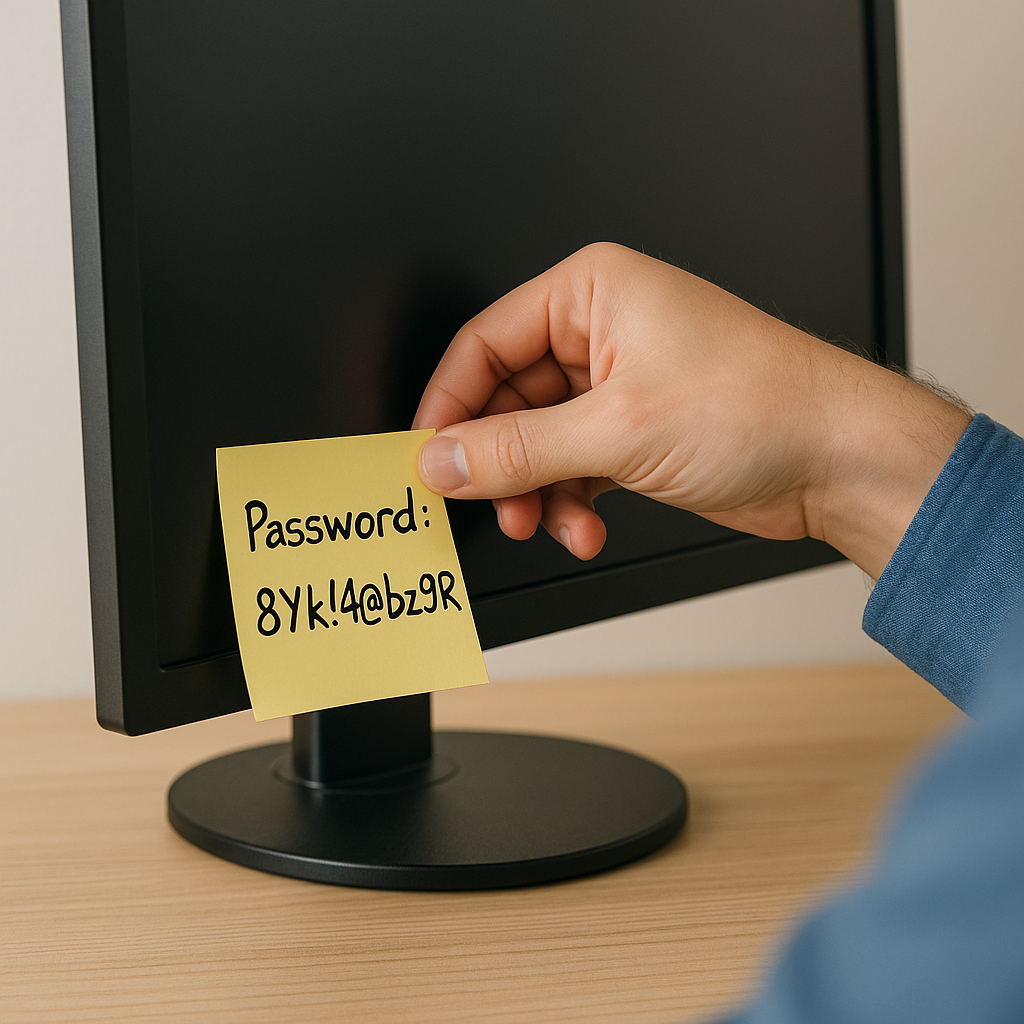
\includegraphics[width=0.9\linewidth]{figures/ai_stick_note.png}
        \caption{\small Generated by AI}
      \end{figure}
    \end{column}
  \end{columns}
\end{frame}
%% -------------------------------------------------------
\begin{frame}{What About Passphrases?}
  \begin{center}
    {\Huge\ttfamily this is a strong password}
  \end{center}
\end{frame}
%% -------------------------------------------------------
\begin{frame}{Enter The Passphrase!}
  \begin{center}
    {\Large \ttfamily this is a strong password}
  \end{center}
  \begin{itemize}
    \item Passphrases are easier to remember and just as strong.
    \item They've become the best practice for humans typing passwords.
    \item Problem solved? Not quite\ldots
  \end{itemize}
  
  \vspace{0.5cm}
  
  \begin{table}[h]
    \centering
    \begin{tabular}{|l|c|c|}
      \hline
      \textbf{Metric} & \textbf{Passphrase} & \textbf{Random Password} \\
      & \texttt{this is a strong password} & \texttt{Lw7@NcQhZ\#f8GvXsT2rY} \\
      \hline
      Charset Size & 58 & 94 \\
      \hline
      Shannon Entropy & 86.49 bits & 86.44 bits \\
      \hline
      Combinations & $1.22 \times 10^{44}$ & $2.90 \times 10^{39}$ \\
      \hline
    \end{tabular}
    \caption{Entropy comparison of a passhphrase and a random password.}
  \end{table}
  
  \centering
  \textbf{Both are equally secure!}\footnote{\tiny Ref: https://alecmccutcheon.github.io/Password-Entropy-Calculator/}
  \vspace{2mm}
\end{frame}
%% -------------------------------------------------------
\begin{frame}
    \vfill
    \centering
    {\bfseries \large Passphrases are strong and memorable, but are they truly secure in every environment?}
    \vfill
\end{frame}
%% -------------------------------------------------------
\begin{frame}{They Can Still Be Stolen}
    \begin{columns}[c]
        \begin{column}{0.3\textwidth}
            \begin{figure}
                \centering
                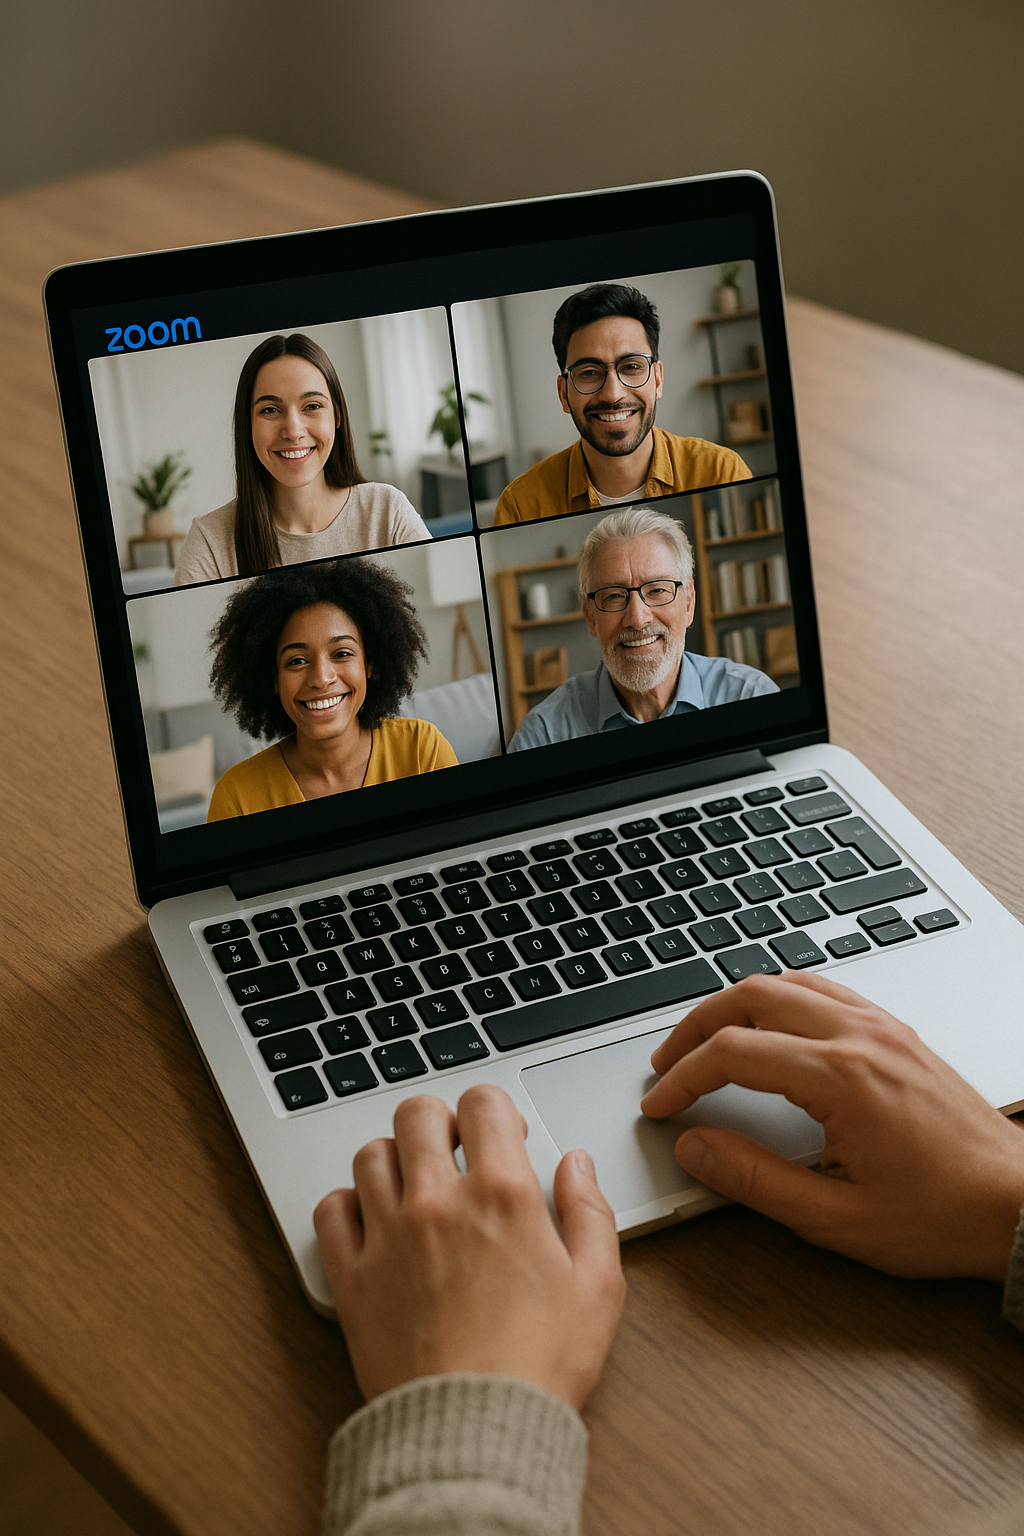
\includegraphics[width=0.8\linewidth]{figures/ai_zoom.png}
                \caption{\small Generated by AI}
            \end{figure}
        \end{column}

        \begin{column}{0.7\textwidth}
            \begin{itemize}
                \item Even your passphrase isn’t safe if someone is listening.
                \item Acoustic Side-Channel Attacks (ASCAs) exploit the sound of your keyboard.
                % \item But they’ve always had one big weakness: noise.
            \end{itemize}
        \end{column}
    \end{columns}
\end{frame}
%% -------------------------------------------------------
\begin{frame}{The Attacker’s Setup Is Simple}
    \begin{figure}
        \centering
        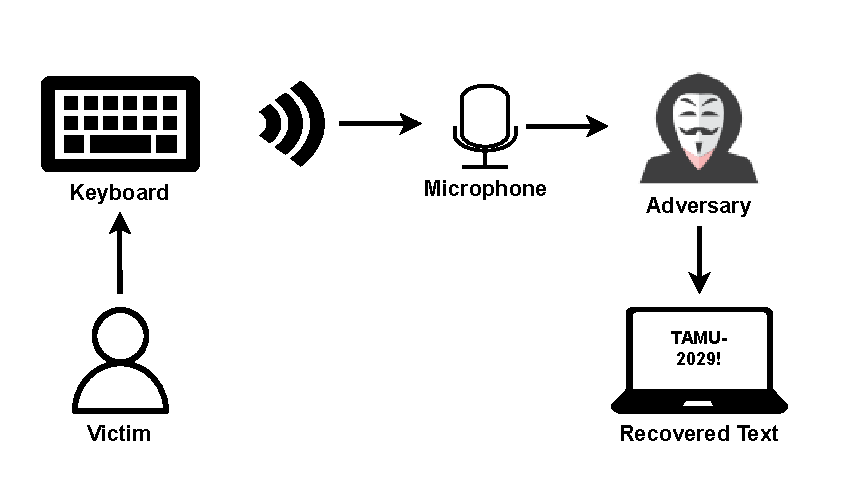
\includegraphics[width=0.65\linewidth]{figures/threat_model.pdf}
        \caption{\small The attacker doesn’t need access to your device. Just a recording—from a call or a nearby phone.}
    \end{figure}
\end{frame}
%% -------------------------------------------------------
\begin{frame}
    \vfill
    \centering
    {\bfseries \large If the setup is simple, what's stopping attackers from succeeding in real-world scenarios?}
    \vfill
\end{frame}
%% -------------------------------------------------------
\subsection{The Challenge of Noise in ASCAs}
\begin{frame}{But...}
    \begin{figure}
        \centering
        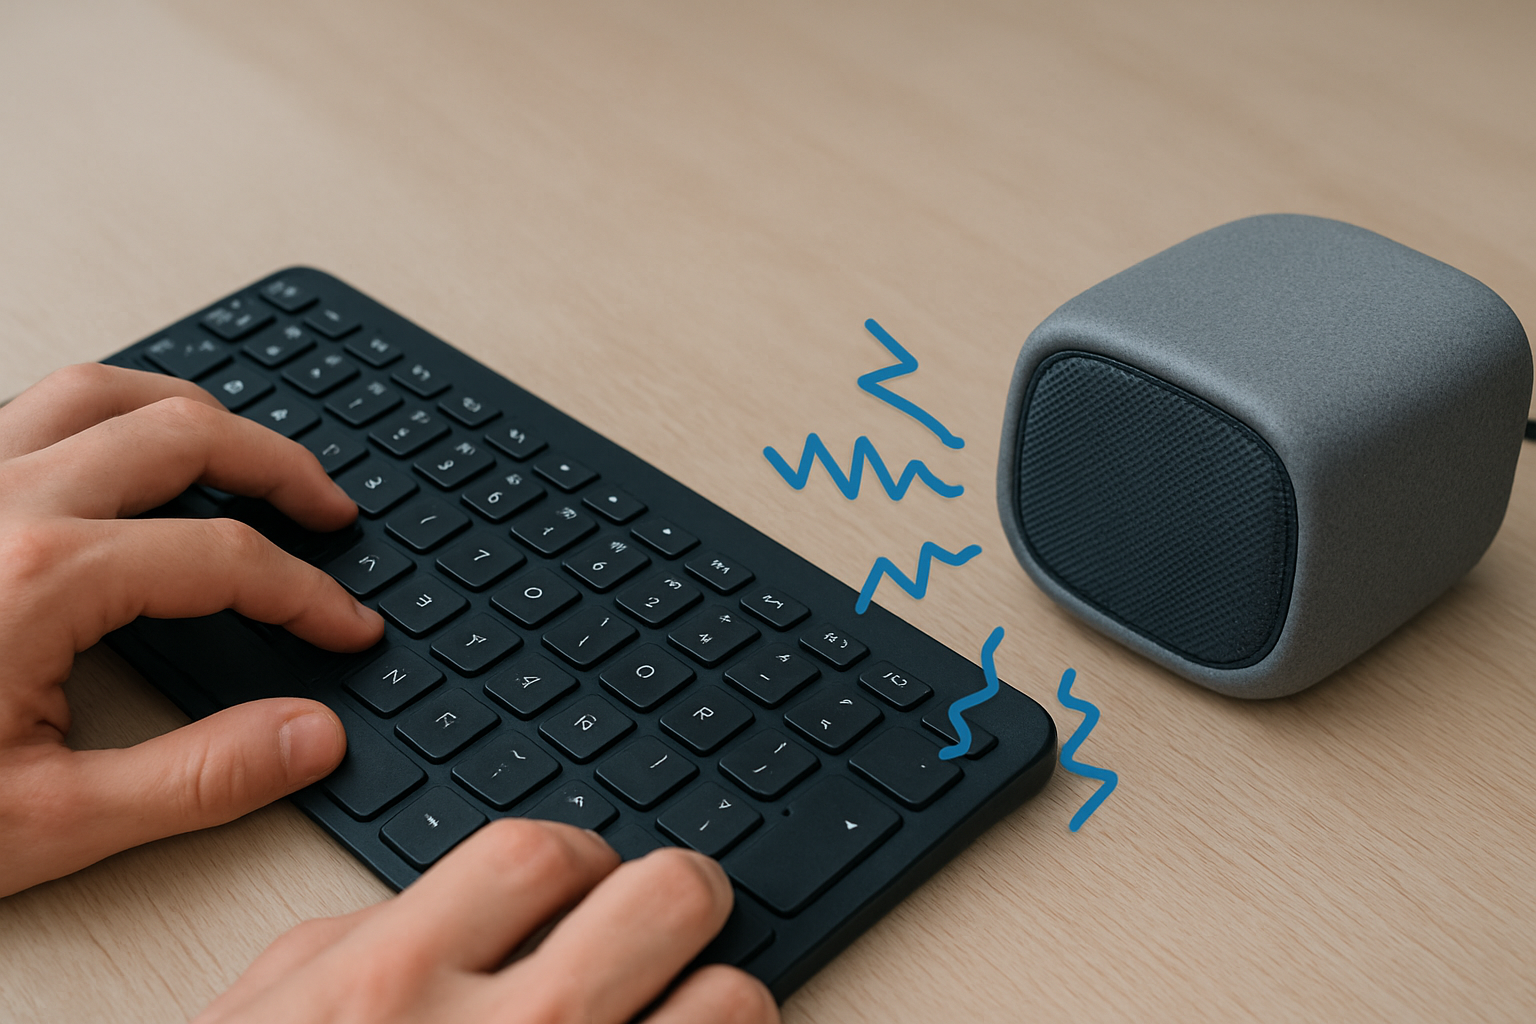
\includegraphics[width=0.5\linewidth]{figures/ai_noise.png}
        \caption{\small ASCAs on keyboards always had one big weakness: \alert{noise}.~\footnote{AI-Generated}}
        \label{fig:enter-label}
    \end{figure}
\end{frame}
%% -------------------------------------------------------
% \begin{frame}{A Brief History}
% \begin{figure}
%     \centering
%     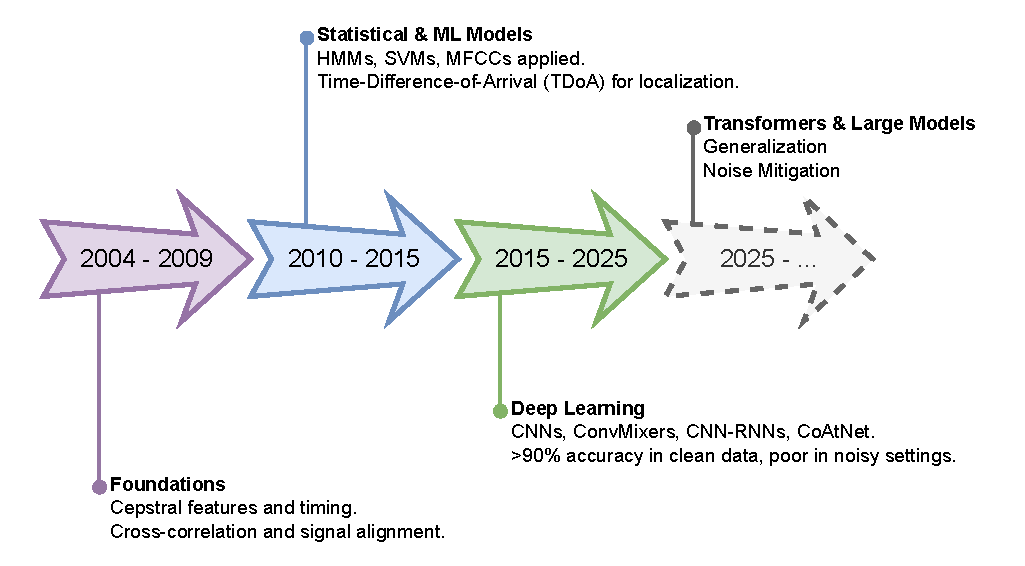
\includegraphics[width=0.75\linewidth]{figures/timeline.pdf}
%     \caption{History of ASCAs on Keyboards}
% \end{figure}
% \end{frame}
%% -------------------------------------------------------
\section{Problem Statement}
\subsection{Noise and Its Impact on Spectrograms}
\begin{frame}{Noise Destroys The Features}
  \begin{figure}
    \centering
    \begin{subfigure}[b]{0.48\textwidth}
        \centering
        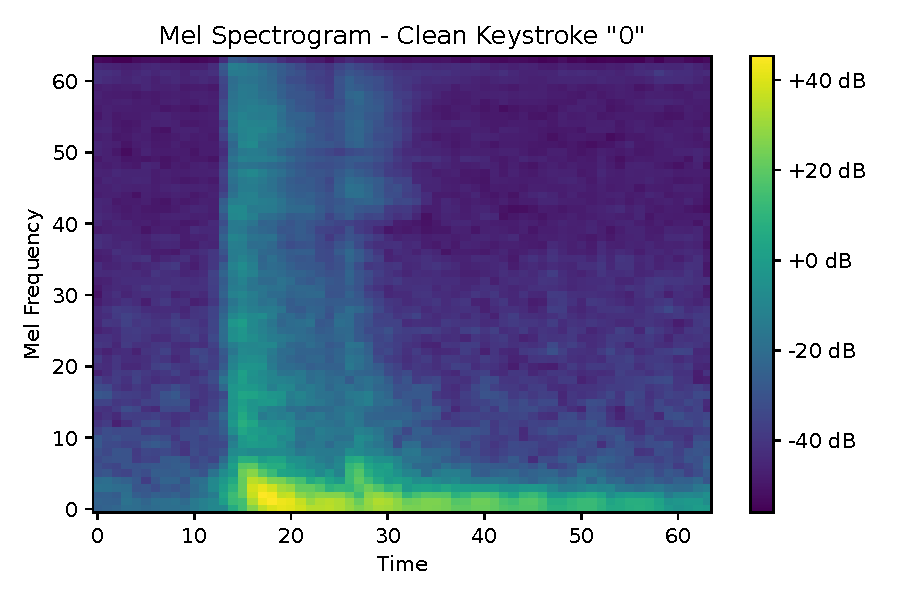
\includegraphics[width=\linewidth]{figures/spectrogram_clean.pdf}
        \caption{\small Clean Spectrogram}
    \end{subfigure}
    \hfill
    \begin{subfigure}[b]{0.48\textwidth}
        \centering
        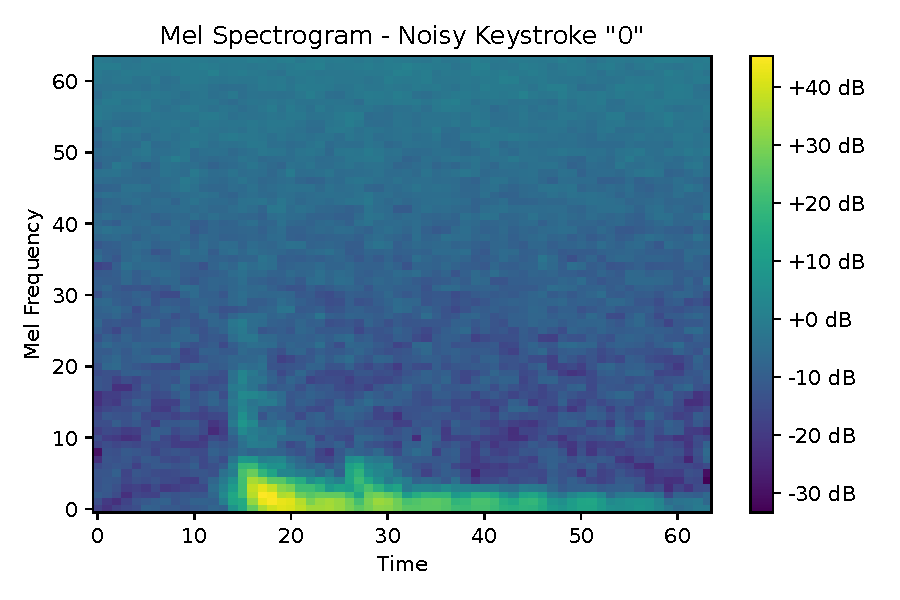
\includegraphics[width=\linewidth]{figures/spectrogram_noisy.pdf}
        \caption{\small Noisy Spectrogram}
    \end{subfigure}
    \caption{(a) and (b) show clean and noisy spectrograms, respectively. Light noise ($10\%$) masks the distinctive keystroke patterns.}
    \label{fig:clean_vs_noisy_spectrogram}
  \end{figure}

  \vspace{1em}
  In noisy environments, the distinctive patterns corresponding to each keystroke are blurred or masked, making direct classification highly unreliable.
\end{frame}
%% -------------------------------------------------------
\subsection{Limitations of Current Models}
\begin{frame}{Even the Best Models Fail Under Noise}
  \begin{figure}
    \centering
    \begin{subfigure}[b]{0.48\textwidth}
        \centering
        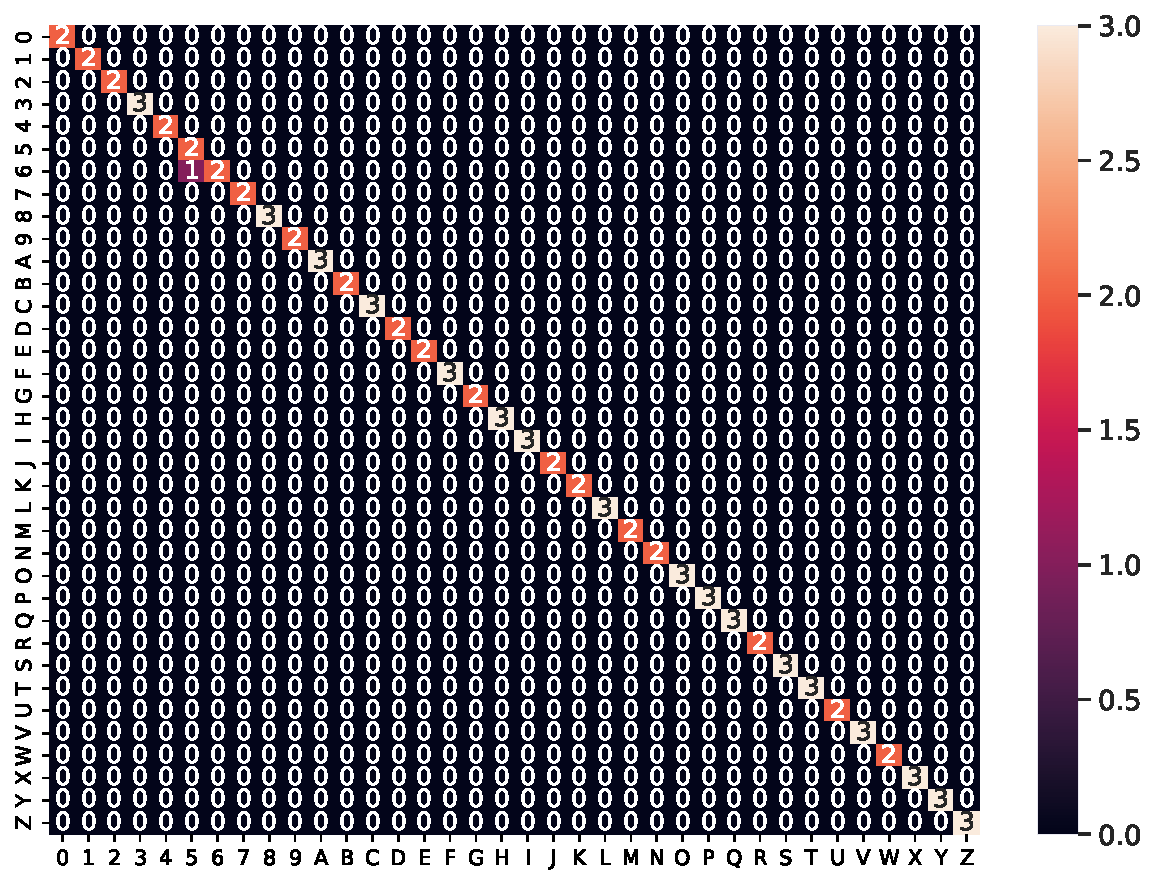
\includegraphics[width=\linewidth]{figures/confusion_clean.pdf}
        \caption{\small CoAtNet on clean audio (\textbf{99\%} accuracy)}
    \end{subfigure}
    \hfill
    \begin{subfigure}[b]{0.48\textwidth}
        \centering
        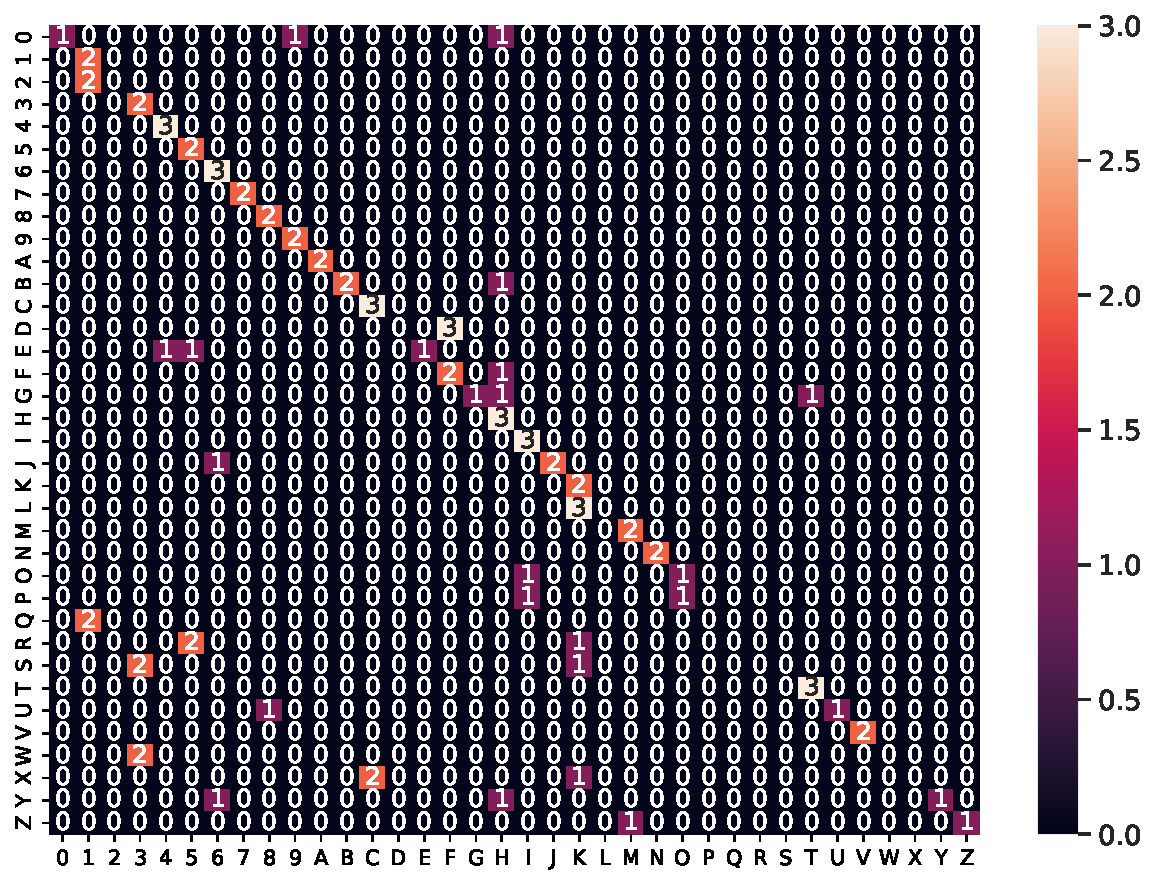
\includegraphics[width=\linewidth]{figures/confusion_noisy.pdf}
        \caption{\small CoAtNet on noisy audio (\textbf{58\%} accuracy)}
    \end{subfigure}
    \caption{(a) and (b) show the confusion matrices of CoAtNet on clean and noisy audio, respectively.}
    \label{fig:confusion_clean_vs_noisy}
  \end{figure}

  \vspace{1em}
  \structure{Problem:} Even state-of-the-art models like CoAtNet suffer major performance drops when spectrograms are noisy.
\end{frame}
%% -------------------------------------------------------
\begin{frame}
    \vfill
    \centering
    {\bfseries \large What if we change the model? Will VTs help?}\\
    {\bfseries \large If the best models struggle, how can we make ASCAs viable in noisy conditions?}
    \vfill
\end{frame}
%% -------------------------------------------------------
\section{Methodology}
\subsection{High‑Level Pipeline}
\begin{frame}{Split the Problem}
  \begin{figure}[ht]
    \centering
    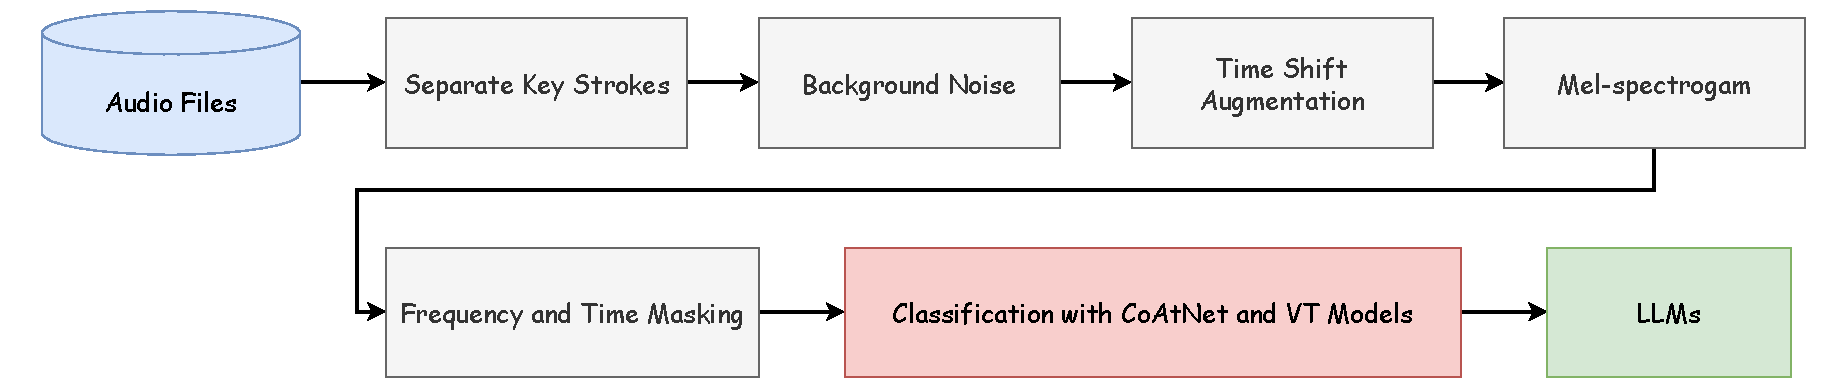
\includegraphics[width=0.9\linewidth]{figures/pipeline.pdf}
    \caption{
      After preprocessing, a Vision Transformer (e.g., Swin) or CoAtNet classifies individual keystroke spectrograms, producing a sequence of noisy character predictions; then, a Large Language Model (e.g., GPT‑4o or LLaMA) corrects transcription errors to produce clean, intelligible text.
    }
    \label{fig:two_stage_pipeline}
  \end{figure}
\end{frame}
%% -------------------------------------------------------
\begin{frame}{Before and After: The LLM Fixes It}
\begin{figure}
    \centering
    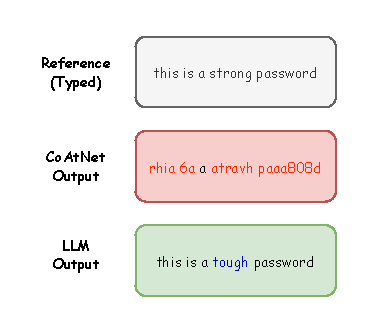
\includegraphics[width=0.45\linewidth]{figures/example_2.pdf}
    \caption{\small The initial text sequence (top) represents the ideal output. The noisy prediction (bottom) introduces typographical
and semantic errors due to environmental noise or model inaccuracies.}
\end{figure}    
\end{frame}
%% -------------------------------------------------------
\subsection{Stage 1: Keystroke Detection with Vision Transformers}
\begin{frame}{Stage 1: Spectrogram $\rightarrow$ Character (Keystroke Detection)}
\begin{figure}
    \centering
    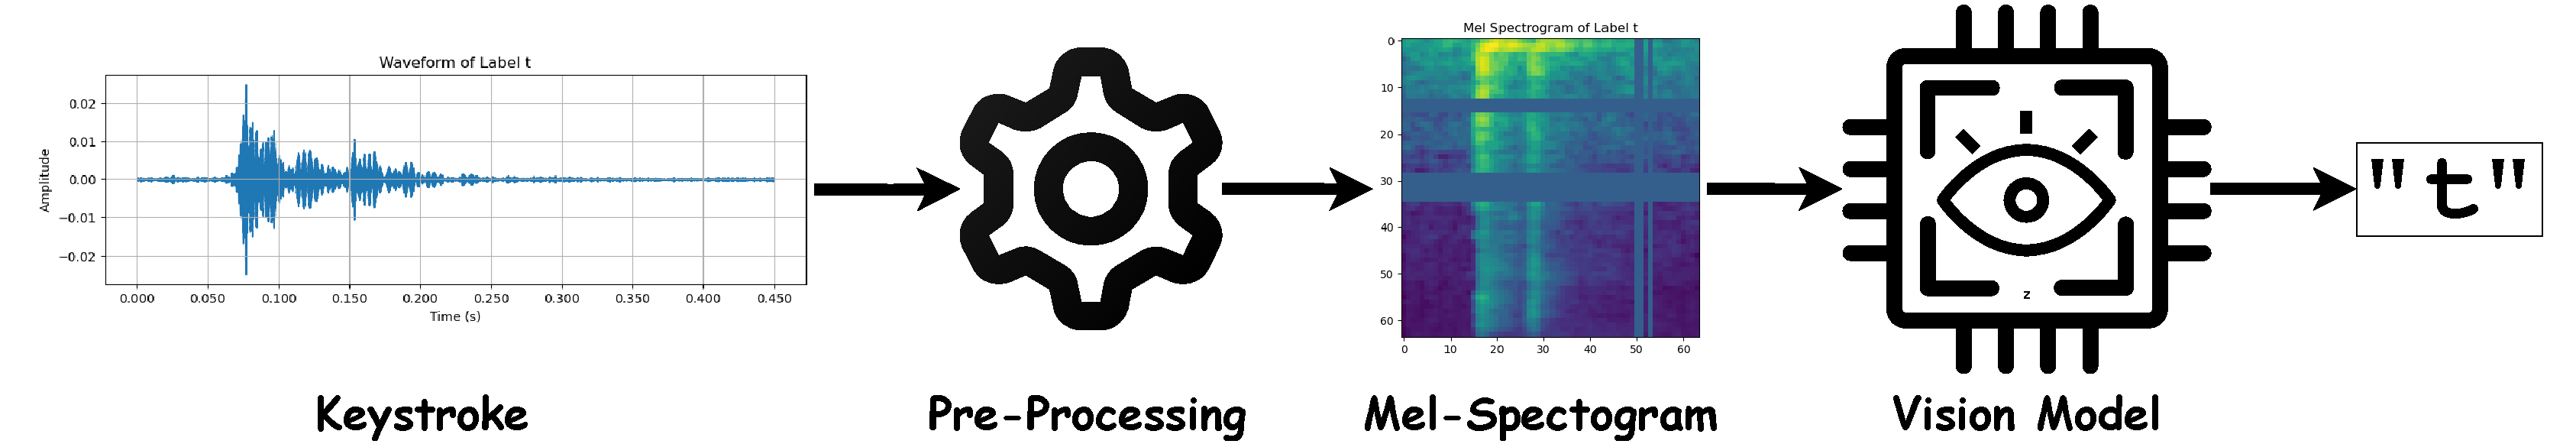
\includegraphics[width=0.95\linewidth]{figures/stage_1.pdf}
    \caption{\small Stage 1}
\end{figure}
  \begin{itemize}
    \item \textbf{Pre-Processing:} Time-shift, time/freq masking data augmentation, transforming into 64x64 mel-spectrogram.
    \item \textbf{Vision Models:} CoAtNet (Baseline), Vision Transformers (ViT, Swin, DeiT, CLIP, BEiT)
    \item \textbf{Datasets:} Zoom, Phone (36 keys $\times$ 25)
  \end{itemize}
\end{frame}
%% -------------------------------------------------------
\begin{frame}{Stage 1: Key Results}
    \begin{minipage}{0.55\linewidth}
        \centering
        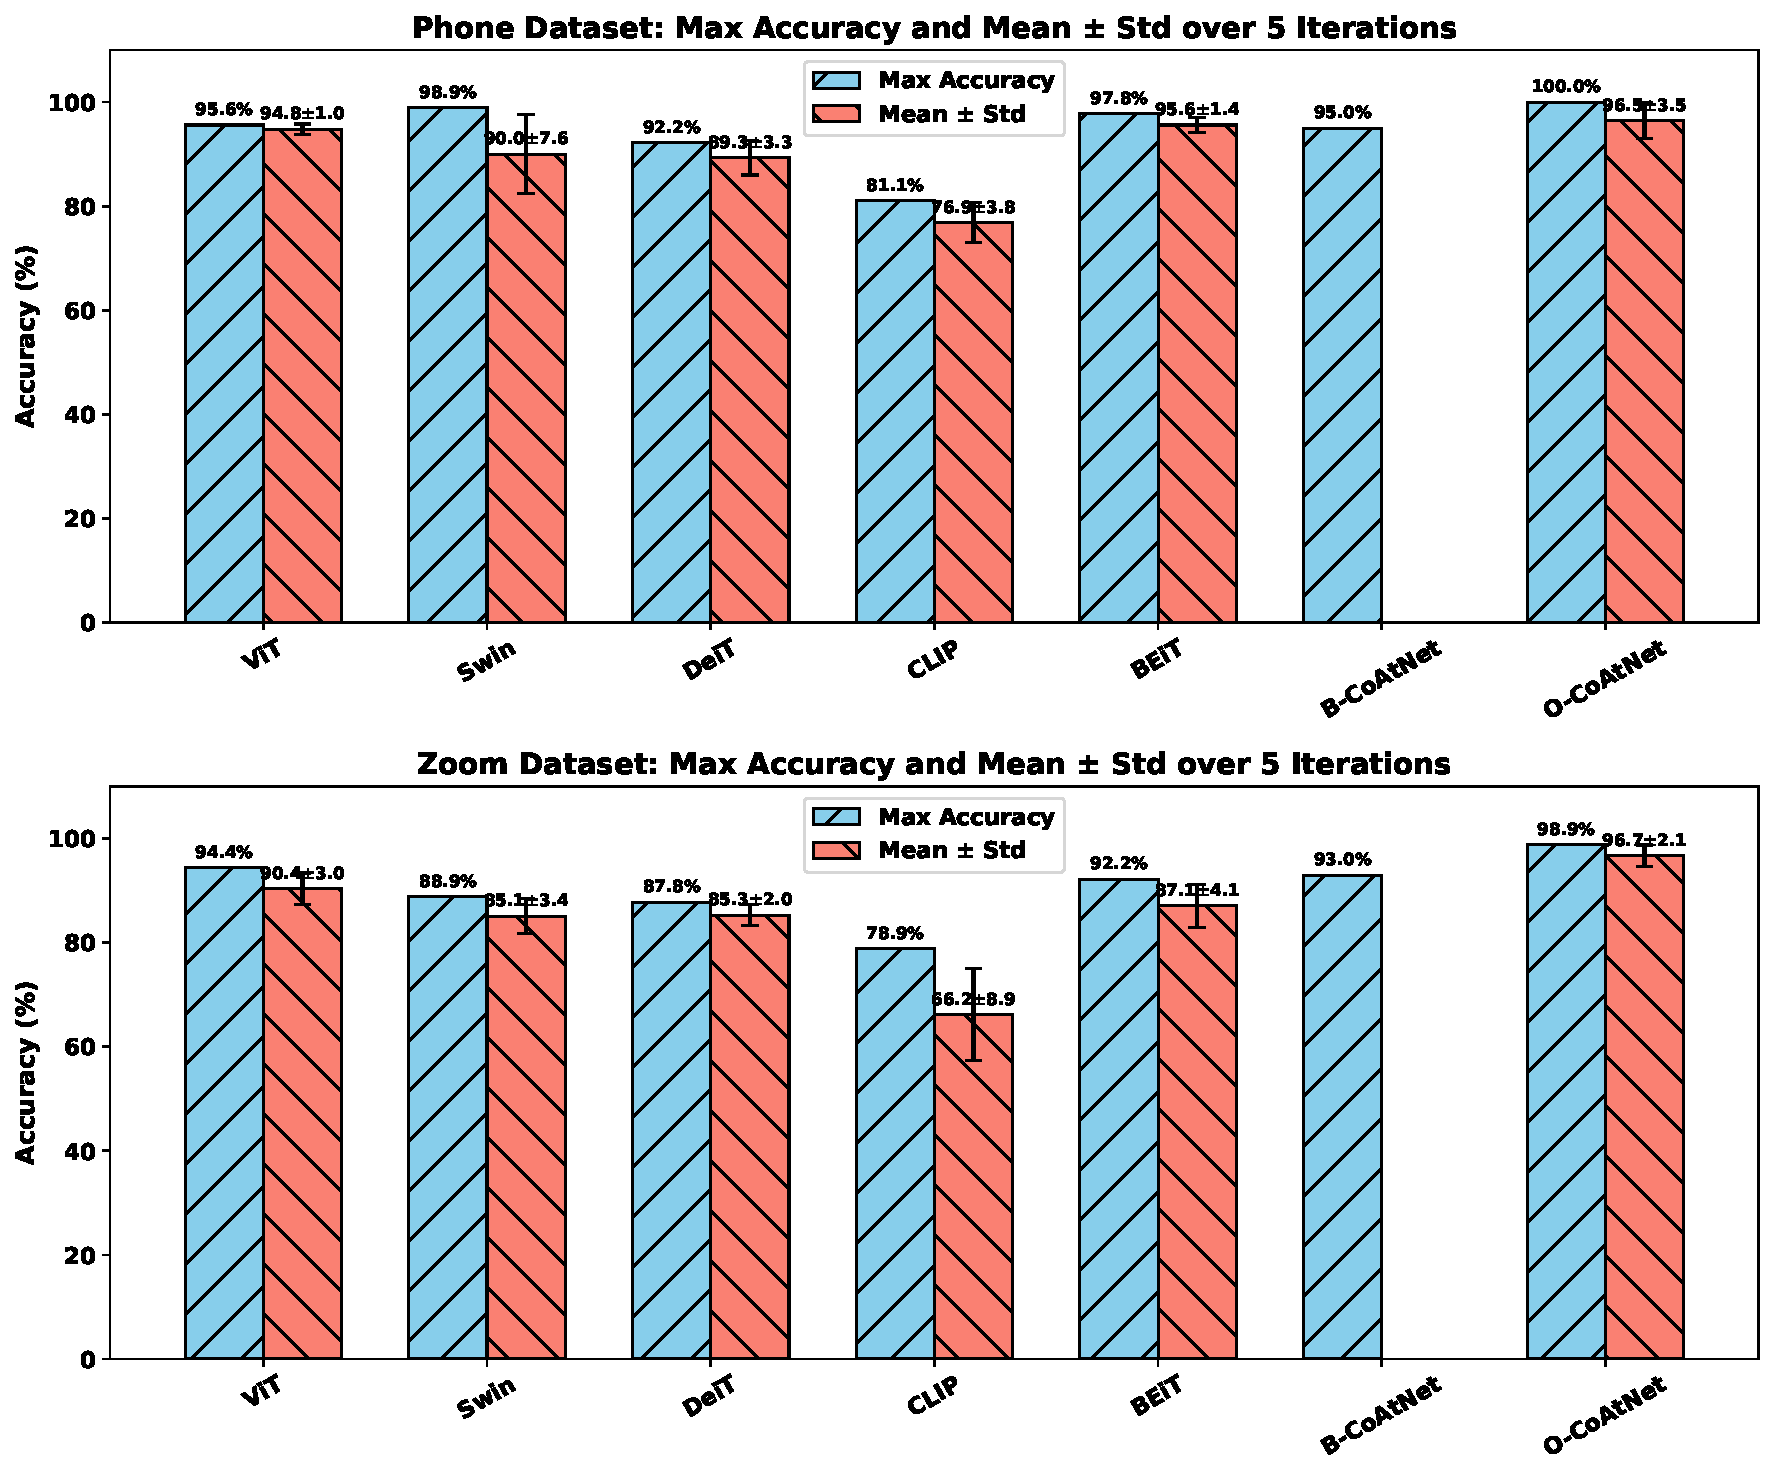
\includegraphics[width=\linewidth]{figures/model_accuracy_comparison.pdf}
    \end{minipage}%
    \hfill
    \begin{minipage}{0.4\linewidth}
        \small
        \captionof{figure}{This plot compares max and average accuracies of different models on the Phone dataset. Max values are in blue, mean ± std in red. \\}
        \vspace{1em}
        \textbf{Highlights:}
        \begin{itemize}
            \item O-CoAtNet achieves highest scores.
            \item CLIP consistently underperforms.
            \item BEiT and Swin show strong accuracy.
        \end{itemize}
    \end{minipage}
\end{frame}
%% -------------------------------------------------------
\subsection{Stage 2: LLM-Based Typo Correction}
\begin{frame}{Stage 2: LLM for Context-Aware Correction}
    \begin{columns}
        \begin{column}{0.7\textwidth}
            \begin{itemize}
                \item Gaussian noise is added to the dataset at varying levels.
                \item Models make mistakes (accuracy drops) due to the noise.
                \item The output sequences often contain typos and, in some cases, are unreadable.
                \item Can an LLM fix this?
            \end{itemize}
            \vspace{-3mm}
            \begin{table}[h]
                \centering
                \caption{Noise factor ($\eta$) applied to each dataset: low, medium, and high correspond to approximately 10\%, 20\%, and 50\% accuracy reductions, respectively.}
                \begin{tabular}{l|ccc}
                    \toprule
                    \textbf{Dataset} & \multicolumn{3}{c}{\textbf{Noise factor ($\eta$)}} \\ 
                                     & \textbf{Low} & \textbf{Medium} & \textbf{High} \\ \midrule
                    Phone            & 0.012        & 0.024           & 0.06          \\ 
                    Zoom             & 0.1          & 0.5             & 1.0           \\ 
                    \bottomrule
                \end{tabular}
            \end{table}
        \end{column}

        \begin{column}{0.3\textwidth}
            \begin{figure}
                \centering
                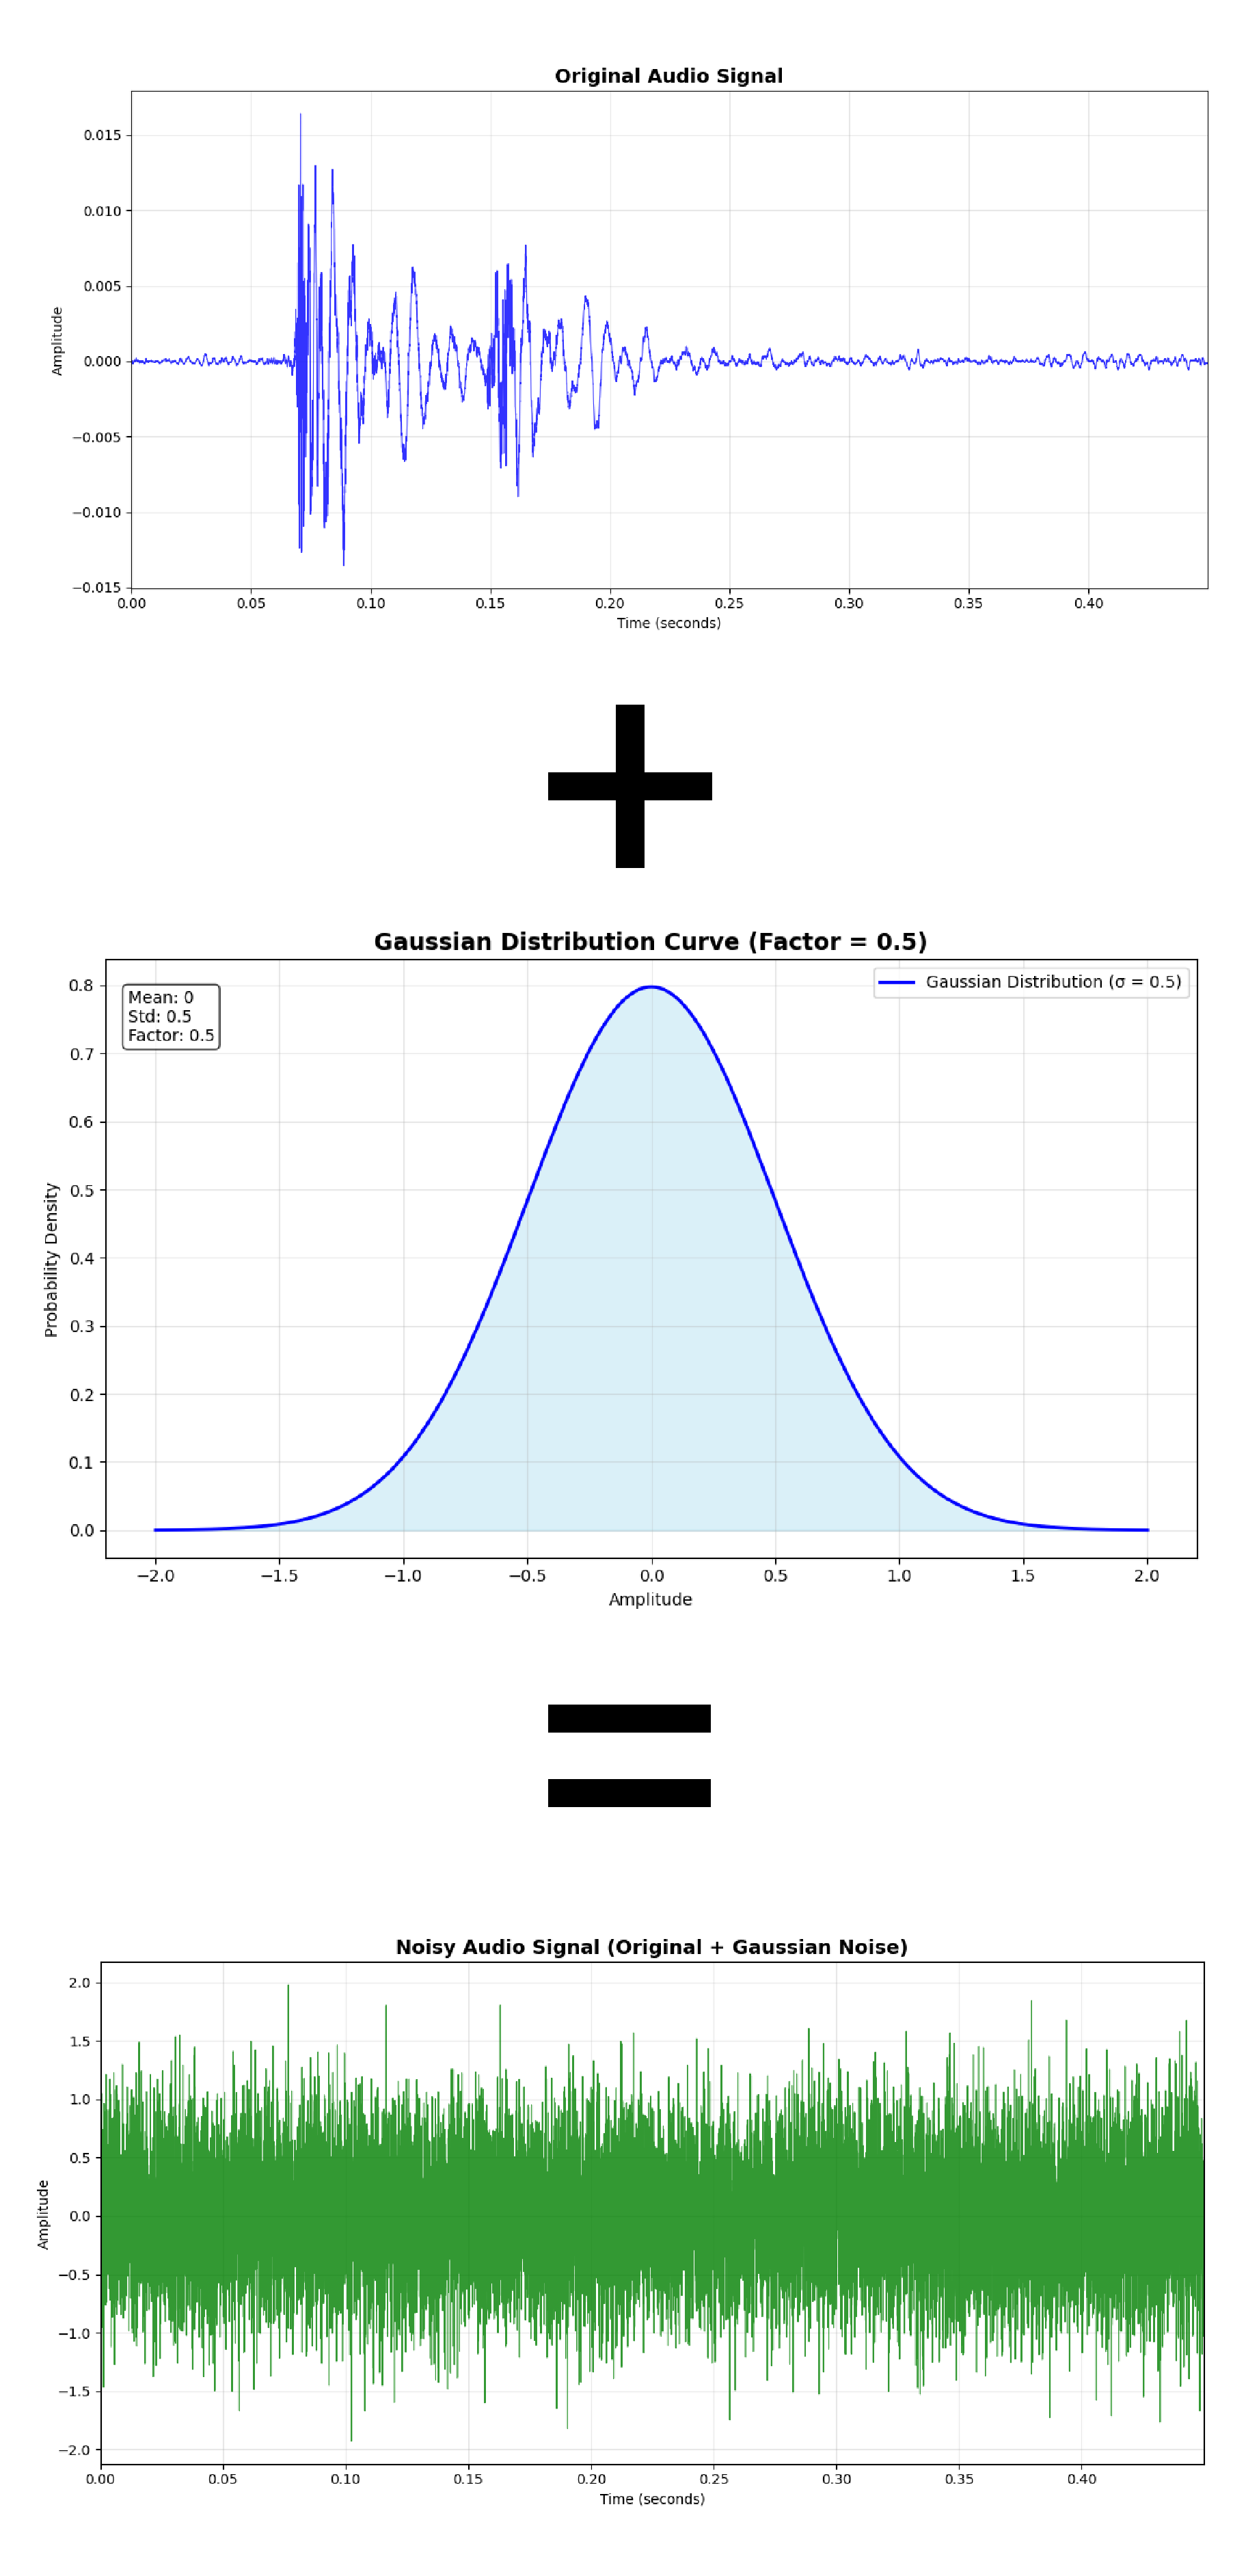
\includegraphics[width=0.75\linewidth]{figures/noise.pdf}
                \caption{Caption}
                \label{fig:enter-label}
            \end{figure}
        \end{column}
    \end{columns}
\end{frame}
%% -------------------------------------------------------
\begin{frame}{Stage 2: LLM Prompt Structure}
    \small
    
    \textbf{System Role:} \\
    \textit{You are an expert in correcting typos in sentences.}
    
    \vspace{1em}
    
    \textbf{User Role:} \\
    \textit{Here are pairs of sentences with typos; learn from them:}
    
    \vspace{0.5em}
    
    \texttt{sentence: \{ $S^{1}_{\text{pred}}$ \}} \\
    \texttt{corrected: \{ $S^{1}_{\text{true}}$ \}}
    
    \vspace{0.5em}
    
    \texttt{sentence: \{ $S^{2}_{\text{pred}}$ \}} \\
    \texttt{corrected: \{ $S^{2}_{\text{true}}$ \}}
    
    \vspace{1em}
    
    \textit{Now, please correct these sentences and output only the corrected version with no additional text:}
    
    \vspace{0.2em}
    \texttt{\{ $S_{\text{pred}}$ \}}
    
    \vspace{1em}
    \begin{block}{Intuition}
        \textit{This few-shot prompt guides the LLM to learn correction patterns and apply them to a new input.}
    \end{block}
\end{frame}
%% -------------------------------------------------------
\begin{frame}{Stage 2: Evaluation Metrics}
    \small
    \begin{block}{BLEU}
        Measures \textbf{precision} of overlapping n-grams (1–4) between model output and reference.
        Penalizes overly short outputs.
    \end{block}
    \begin{block}{METEOR}
        Uses \textbf{precision + recall} with flexible matching (stems, synonyms, paraphrases) and a penalty for word order differences.
    \end{block}
    \begin{block}{ROUGE-1 / ROUGE-2}
        Recall-oriented: counts overlapping unigrams (ROUGE-1) or bigrams (ROUGE-2), capturing vocabulary coverage and short phrase accuracy.
    \end{block}
    \begin{block}{ROUGE-L}
        Based on the \textbf{longest common subsequence} between output and reference, reflecting structural similarity and word order.
    \end{block}
\end{frame}
%% -------------------------------------------------------
\begin{frame}{Stage 2: Key Results}
    \begin{figure}
        \centering
        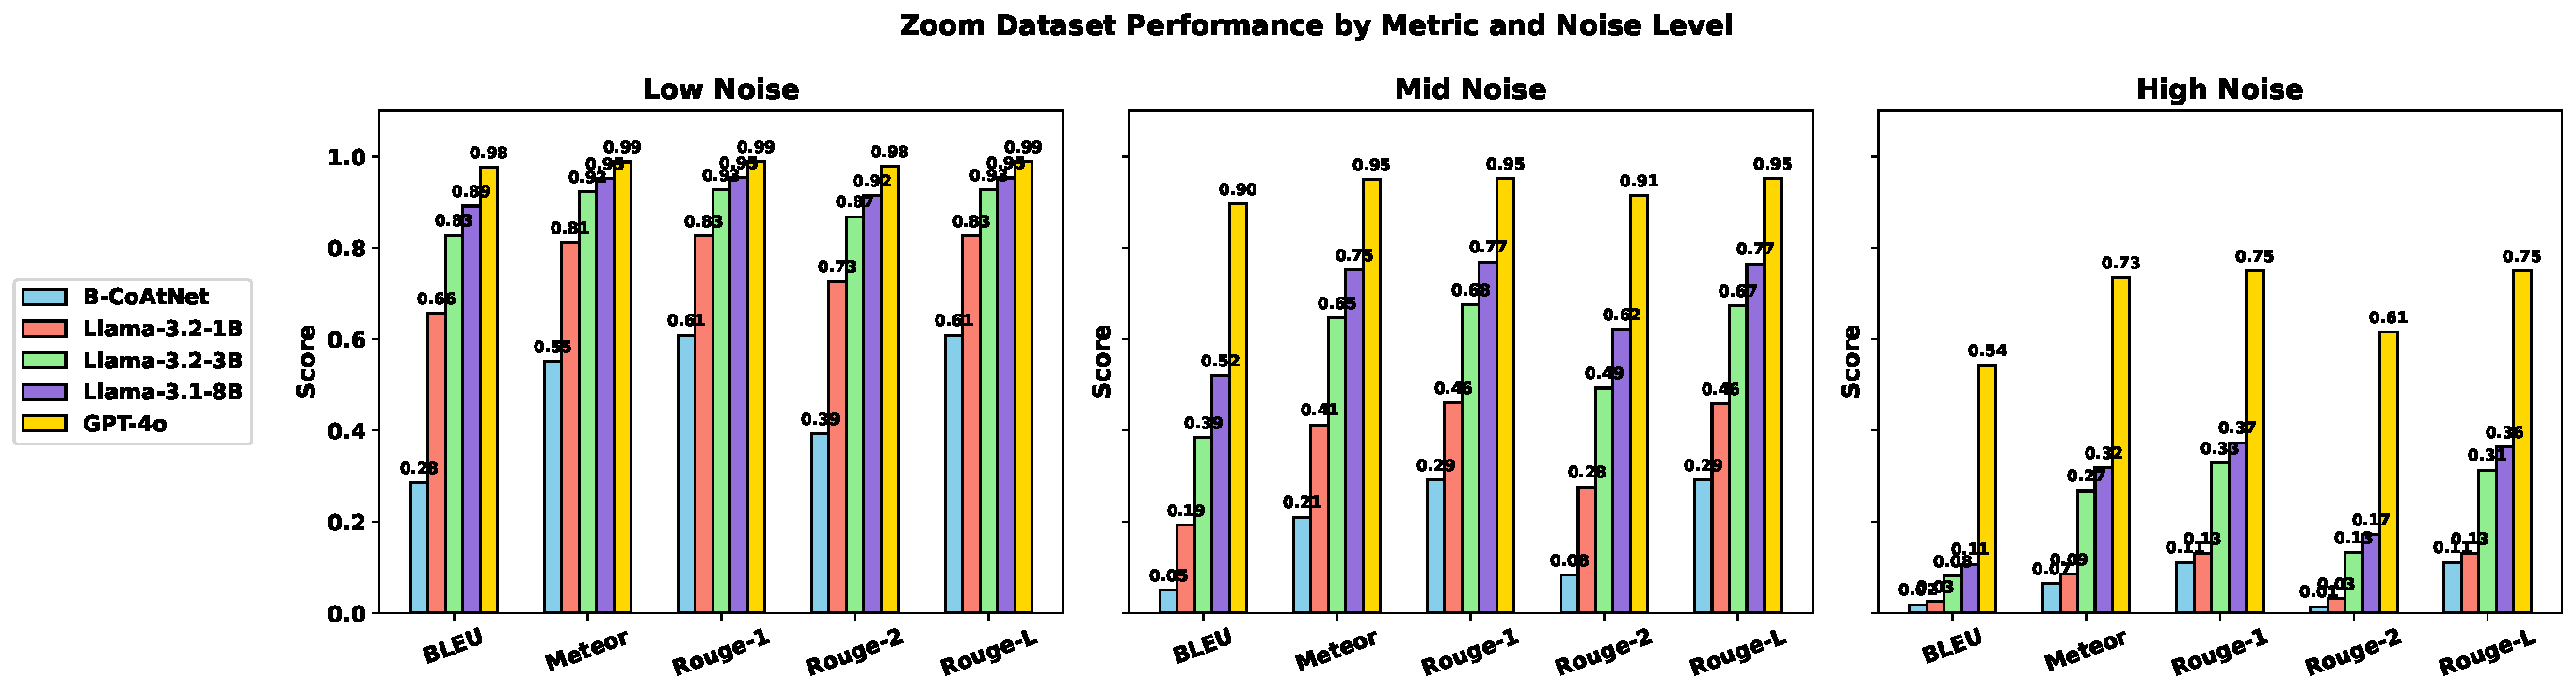
\includegraphics[width=0.95\linewidth]{figures/llm_zoom_performance.pdf}
        \caption{\small Performance of various models on the Zoom dataset across BLEU, METEOR, and ROUGE metrics under different noise levels. GPT-4o consistently outperforms smaller models, especially under high noise conditions.}
        \label{fig:llm-zoom-performance}
    \end{figure}
\end{frame}
%% -------------------------------------------------------
\begin{frame}

    \vfill
    \centering
    {\bfseries \large GPT-4o outperforms all models. We cannot use it offline, and other big models are resource intensive. Can we achieve the same performance with a much smaller model?}
    \vfill
    
\end{frame}
%% -------------------------------------------------------
\subsection{Smaller Models for Practical Attacks}
\begin{frame}{Can Smaller Models Match the Giants?}
    \begin{block}{The Challenge}
        While \textbf{LLaMA-3.1-8B} and \textbf{GPT-4o ($\sim200B$)} achieve state-of-the-art performance,
        they are:
        \begin{itemize}
            \item Resource-intensive (need 16–30+ GB RAM/VRAM)
            \item Impractical for low-resource or stealthy attack scenarios
            \item Expensive to deploy at scale
        \end{itemize}
    \end{block}

    \vspace{0.8em}

    \begin{block}{Our Goal}
        Investigate whether a much smaller model, like \textbf{LLaMA-3.2-3B}, can be:
        \begin{itemize}
            \item Fine-tuned or prompted effectively
            \item Competitive in performance with large models
            \item Suitable for practical, real-world attacks
        \end{itemize}
    \end{block}
\end{frame}
%% -------------------------------------------------------
\begin{frame}{Small Model, Big Results}
    \begin{figure}
        \centering
        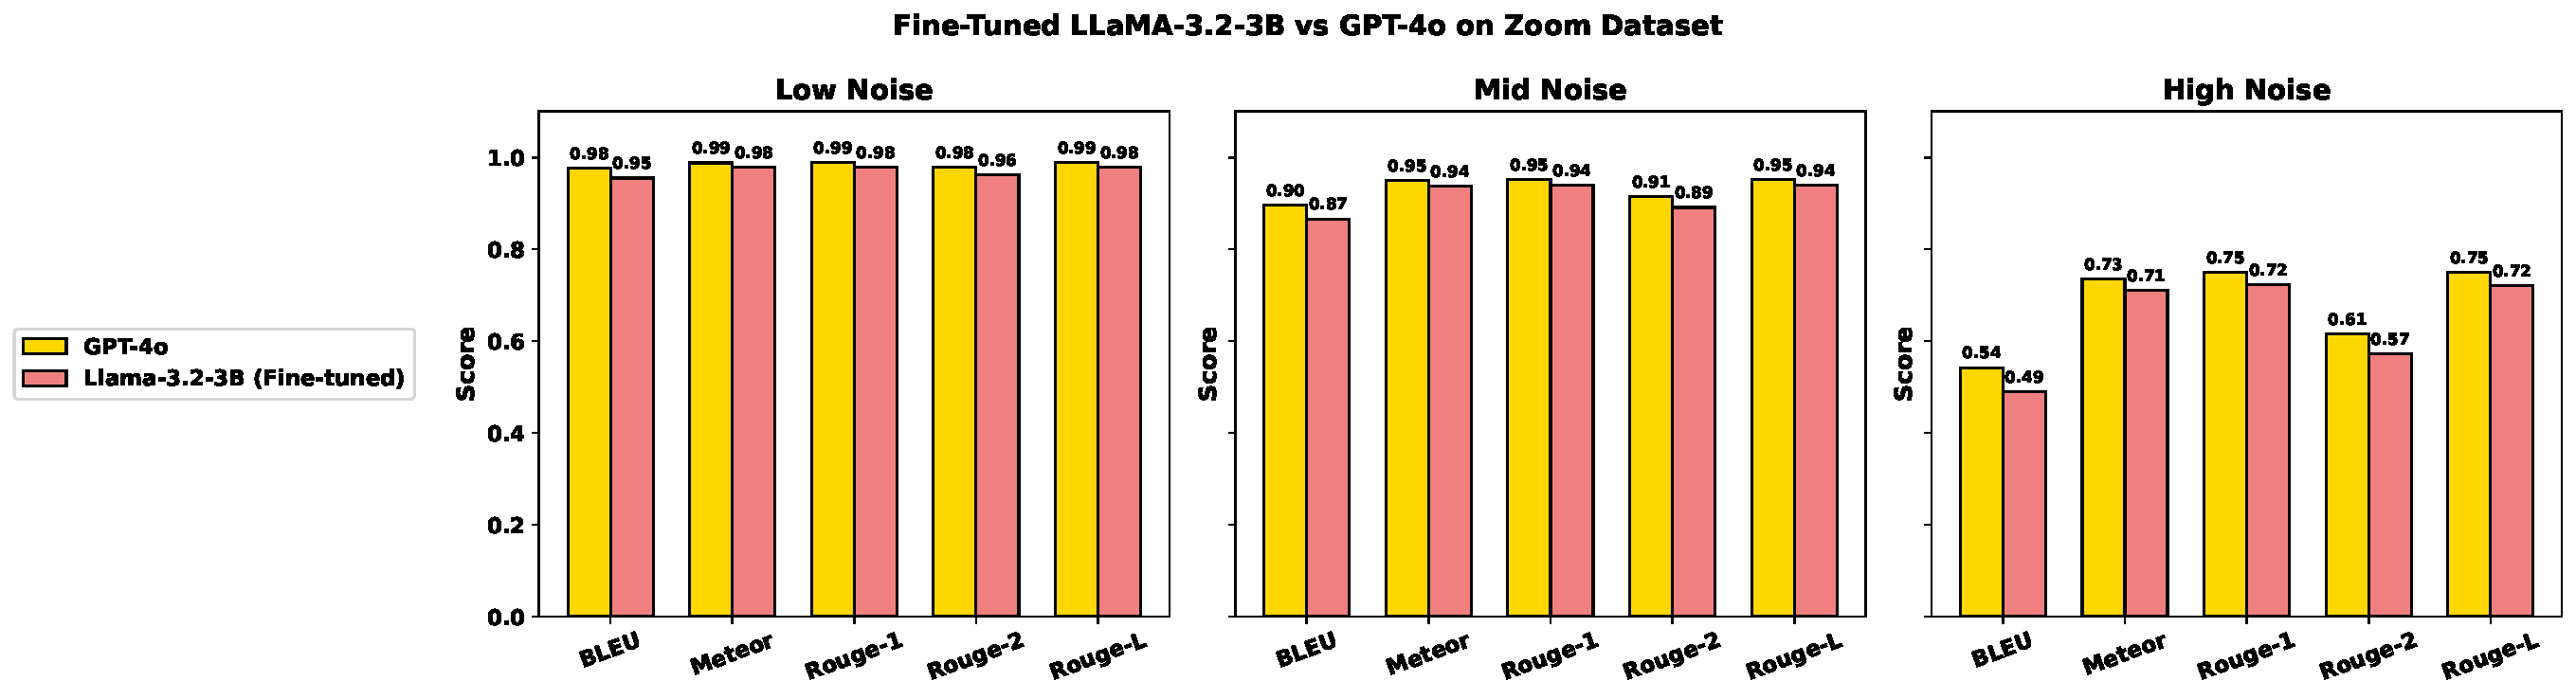
\includegraphics[width=0.95\linewidth]{figures/ft_zoom_performance.pdf}
        \caption{\small GPT-4o vs fine-tuned LLaMA-3.2-3B (LoRA) across metrics and noise levels on the Zoom dataset.}
        \label{fig:ft_zoom}
    \end{figure}

    \vspace{0.5em}
    \centering
    \alert{\textbf{→ Achieves ~90\% of GPT‑4o performance with ~1.5\% of its model size.}}
\end{frame}
%% -------------------------------------------------------
\section{Conclusion}
\subsection{Limitations and Future Work}
% \begin{frame}{Limitations \& Future Work}
%   \begin{block}{Current Limitations}
%     \begin{itemize}
%       \item \textbf{Dataset Size:} Only 36 keys and 25 repetitions; no space or backspace events.
%       \item \textbf{Noise Profile:} Synthetic Gaussian noise used $\Rightarrow$ does not fully represent real-world ambient noise.
%       \item \textbf{Hardware Diversity:} Evaluated on a single device (MacBook Pro); cross-device generalization is still a challenge.
%     \end{itemize}
%   \end{block}

%   \vspace{0.5em}

%   \begin{block}{Future Work}
%     \begin{itemize}
%       \item Expand to larger, open-access datasets.
%       \item Record and evaluate under real ambient noise conditions.
%       \item Support real-time, on-device inference and model portability.
%     \end{itemize}
%   \end{block}
% \end{frame}
\begin{frame}{Limitations \& Future Work}
  \begin{block}{Field-Wide Gaps}
    \begin{itemize}
      \item \textbf{Dataset Availability:} Public ASCA datasets are tiny (36 keys, no space/backspace), limiting what any research can currently test.
      \item \textbf{Noise Realism:} Community datasets lack real-world ambient noise — most use synthetic Gaussian noise as a proxy.
      \item \textbf{Hardware Diversity:} Nearly all public datasets focus on a single device type (e.g., MacBook Pro), making cross-device benchmarks rare.
    \end{itemize}
  \end{block}

  \vspace{0.5em}

  \begin{block}{Call to the Community}
    \begin{itemize}
      \item Collaboratively build and release \textbf{large, open-access ASCA datasets}.
      \item Include recordings with realistic ambient noise conditions.
      \item Cover diverse devices and keyboards to enable true generalization.
    \end{itemize}
  \end{block}
\end{frame}

%% -------------------------------------------------------
\subsection{Key Takeaways}
\begin{frame}{Key Takeaways \& Conclusion}
  \begin{block}{What We Showed}
    \begin{itemize}
        \item \textbf{Vision Transformers (VTs)} achieved accuracy close to the current state-of-the-art (CoAtNet), showing strong potential for keystroke spectrogram recognition.
      \item \textbf{LLMs} are essential for handling real-world noise in post-processing.
      \item \textbf{Fine-tuned small models} enable portable and practical attacks.
      \item First end-to-end \textbf{VT + LLM} pipeline for keyboard ASCAs under noise.
      \item Achieved \textbf{$>$95\%} text recovery under medium noise with a small model.
    \end{itemize}
  \end{block}
    \begin{block}{Security Implication}
      Keystrokes can be inferred acoustically—even strong passphrases are vulnerable.\\
      \textbf{Adopt MFA and biometrics to mitigate this risk.}
    \end{block}
\end{frame}

%% -------------------------------------------------------
\section*{Q\&A}
\begin{frame}{Questions?}
  \begin{columns}
    \column{0.75\textwidth}
      \centering
      \Huge\textbf{Thank You!}

      \vspace{0.8cm}
      % \Large\textit{Contact Info:}

      \vspace{0.4cm}
      \normalsize
      \href{mailto:ali.a@tamu.edu}{\texttt{ali.a@tamu.edu}} 
      \(\mid\) 
      \href{https://ali-ayati.com}{\texttt{ali-ayati.com}}

      \vspace{0.5cm}
      \small
      \textit{Slides and code:} \href{https://github.com/Botacin-s-Lab/EchoCrypt}{\texttt{github.com/Botacin-s-Lab/EchoCrypt}}

      \vspace{0.5cm}
      \begin{minipage}{0.95\textwidth}
        \centering
        
\includegraphics[height=1cm]{figures/usenixbadges-available.pdf}\hspace{0.3cm}
        
\includegraphics[height=1cm]{figures/usenixbadges-functional.pdf}\hspace{0.3cm}
        
\includegraphics[height=1cm]{figures/usenixbadges-reproduced.pdf}
      \end{minipage}

    \column{0.25\textwidth}
      \centering
      
\includegraphics[width=0.9\linewidth]{figures/qr_github.png}
  \end{columns}
\end{frame}



\end{document}
